\chapter{INTRODUCTION}
\label{Section: Introduction}

In this work, we consider using passive RFID (radio frequency identification) technology beyond its traditional purpose, that is, identification. Instead, we consider this technology giving rise to \emph{distributed physical information systems}.

\section{Thesis: Exploiting Tag Multiplicity}
\emph{Given existing science and technology trends, passive RFID is a necessary component for, and the unique supporting solution that enables, the design and implementation of continuous pervasive spaces. In particular, we argue that a large number of tags, that is, passive RFID tag multiplicity, allows us to design and deploy robust, distributed physical information systems, achieving this particular goal of pervasivity.} 

In the following, we unpack this thesis statement, explaining what are continuous pervasive spaces and distributed physical information systems. 

\section{Pervasive Computing and Continuous Pervasive Spaces}
Many years ago, Mark Weiser coined the term \emph{ubiquitous computing} \cite{1991 Weiser}. Today, \emph{pervasive computing} is often used as well. Pervasive computing is concerned with bringing computation to the real physical world, and eventually relieving the everyday user from the awareness of the technology itself \cite{1991 Weiser}.

One particular area of pervasive computing is pervasive spaces. The authors in \cite{2002 Roman} introduce an \emph{active space} as a physical area where human users interact with intelligent devices, thereby augmenting human thought and activity. (We prefer the term \emph{pervasive space} since it draws from pervasive computing.) The physical area could be in the home, office, or a public space. Heterogeneous devices are networked in a distributed fashion. The entire system thus provides users with a pervasive computing environment. The authors in \cite{2002 Roman} provide a middleware platform called \emph{Gaia}, that coordinates the services between devices and human users. In other words, Gaia enables the design and deployment of pervasive spaces. The authors in \cite{2004 Shankar}, \cite{2005 Chetan} refine Gaia to individuals. That is, Mobile Gaia is focused on personal pervasive spaces. It provides services such as automated bootstrapping of a personal space when smart devices are physically near each other. This cluster management service thus coordinates discovery, addition, and removal of devices and applications. At the other end of the spectrum is \emph{Super Spaces} \cite{2004 Al-Muhtadi}. The authors here provide a distributed architecture to enable multiple pervasive spaces to interact with each other. We thus see that pervasive spaces are focused on the interaction between human users and devices. \emph{Devices} increasingly also refers to sensors and sensor-embedded devices. This is a natural evolution of pervasive spaces since a system knowing the physical environment can provide a richer experience to the user.

\subsection{Device-Centric View}
Three key ingredients in these pervasive spaces are (1) communication and data flow, (2) data storage, and (3) computation. (Note that sensing uses all three of these ingredients.) We explain these ideas in further detail later. But for now, consider how different devices fall into a space-time spectrum of these three combined ingredients. That is, more communication in space-time means higher volume of data flowing over a larger period. More data storage in space-time means greater storage capacity, with that capacity maintained over a larger period. And more computation in space-time means increased processing over larger areas and over a larger period. Figure \ref{Figure: Devices_Spectrum.eps} shows devices in a space-time spectrum. Note that we consider devices working individually, or at most in small quantities. When devices (homogeneous or heterogenous) are networked together, the resulting systems are located in different places on the space-time spectrum. In Figure \ref{Figure: Devices_Spectrum.eps}, NFC (near field communication) is placed at the bottom left. NFC is a short range passive technology \cite{NFC}. Active interrogators can only scan NFC tags at a range of a few centimeters, and very little storage is possible in an NFC tag. The communication throughput is also low, operating on the order of hundreds of kilobits per second. Passive RFID technology is of course the main focus of this work. We detail RFID later. Its greater communication range (up to tens of meters) and storage capability allow it to be situated higher in the space-time spectrum, compared with NFC. An active RFID \cite{Active RFID} tag has an on-board battery, allowing it even greater communication, storage, and computation abilities. To be activated, they still have to be scanned by interrogators, so they are still considered RFID. This is in contrast to active sensors (motes), which can initiate their own communications, and as a result, are often continuously part of a sensor network. Passive sensors have to harvest their own energy to sense, and maybe even communicate. They may be attached to RFID tags to alleviate the communication energy burden. At the other extreme of the spectrum, we have smart mobile devices and full-fledged devices with sophisticated communication, data storage, and computation capabilities. Interestingly, there is a significant gap in the spectrum, which we believe is inherently caused by the economics of the various technology industries involved with these devices.

\subsection{Environment-Centric View}
Despite the focus on smart environments in pervasive spaces, existing systems still must take devices into account. Supporting software services have to enable devices to interact with each other. Furthermore, human users are still aware of the presence and heterogeneity of devices, often resulting in added cognitive load, resulting in confusion. For example, a user is very much aware if she is using a small screen mobile device, a medium screen tablet, or a large screen mounted computer. To truly approach an environment-centric view of pervasive spaces where users just live, and not interact directly with devices, there needs to be an increased granularity in the three key ingredients of pervasive spaces. Technology is still inherently discrete (and will remain so for the foreseeable future). This technology discretization leads to an unfulfilled pervasive experience for the human user, since the real physical world is continuous. For example, while watching a video, if a user switches between devices, she is entirely aware of this, especially if the devices are different screen sizes, and even more so if she has to actively re-start the video in the new device. To be truly pervasive, the video could follow the user instead, perhaps being projected onto surfaces such as tables and walls. This shows that although technology is discrete, the user experience can still be continuous. We believe that this can be achieved if the discretization is so highly granular that the user perceives continuity. In Figure \ref{Figure: Granularity_Spectrum.eps}, we consider the space-time granularity spectrum of the key ingredients in systems for pervasive spaces. We see that Super Spaces from \cite{2004 Al-Muhtadi} are not very granular at all, since they focus on coordinating the interactions between multiple pervasive spaces. Mobile Gaia from  \cite{2004 Shankar}, \cite{2005 Chetan} is focused on personal pervasive spaces. They are aimed at enhancing the user experience at an individual level. However, the user is still very much aware of the presence and use of devices. We argue that passive tag-based information systems provide the highly sought after granularity, enabling what we now call \emph{continuous pervasive spaces}, leading to a environment-centric view, instead of a device-centric view of pervasive spaces.

\subsection{Characteristics of Continuous Pervasive Spaces}
\label{Section: Introduction: Pervasive Computing and Continuous Pervasive Spaces: Characteristics of Continuous Pervasive Spaces}
We consider several characteristics of continuous pervasive spaces. Achieving these characteristics in a system is tantamount to arriving at a continuous pervasive space. (1) \emph{Continuous pervasive spaces provide a set of rich services for users.} These services enhance the user's life, rather than introduce additional complexity. In that sense, they are transformative, allowing a user the flexibility to do things otherwise not possible, in a highly productive fashion. (2) \emph{The rich services are elastic in their availability and integrity, according to the availability of resources.} This includes the availability and integrity of system data. (3) \emph{The user is minimally distracted from the technology.} Often these distractions arise from the discretization of the user experience, due to the discrete nature of technology itself. (4) \emph{The system supporting the continuous pervasive space is distributed and scalable.} (5) \emph{It is fault-tolerant.} (6) \emph{It is energy-efficient and cost-efficient, as well as cost-flexible.}

\subsection{Competing Systems and Technologies: Not Sufficiently Continuous}
We discuss how passive RFID is a necessary component for continuous pervasive spaces, from the negative. That is, we show how competing technologies cannot achieve continuity in the absence of passive RFID. Note that in many cases, depending on the particular service or environment, we do need these technologies for pervasivity. However, on their own, they lack the inherent continuity that RFID provides.

NFC is a very cost-efficient solution for identification and authentication, often providing security applications such as physical real-world access control. NFC is also used to bootstrap communications between two devices, since it is a quick way to trade credentials. Subsequent communication takes place using a higher throughput technology. Therefore, we see that the short-range and limited throughput nature of NFC hinders its ability to communicate effectively, especially in comparison to RFID, which has greater range, throughput, and storage capability in its tags.

Active RFID is a more sophisticated technology. Active RFID tags have significant storage capability, can transmit further, and can perform more complex computations. However, this means that an active RFID tag is more expensive, is larger in size, and also requires an on-board battery. Although quite useful, these tags therefore cannot be cost-effectively deployed densely in physical spaces. If such tags fail, or their energy supplies are depleted, they quickly become a burden to replace.

Active sensors also suffer from the energy requirements of active RFID. Deploying motes densely in a physical space and networking them together wirelessly would indeed provide a powerful pervasive system, but only in the short run. It would not be cost-effective to maintain such a system, since over time it would require replacing relatively expensive motes that have failed or that have depleted batteries.

Passive sensors have to harvest energy to sense, and maybe communicate. (Some passive sensing systems use an active entity to collect sensing data at relatively large periodic intervals. But this fails the high time granularity requirement of continuous pervasive spaces.) As a result, sensing and communication are extremely limited, subject to the energy harvesting method and fluctuating conditions, such as absorbing solar energy during unpredictable weather patterns. This violates the requirement of having a high granularity in the key ingredients of a continuous pervasive space.

Finally, smart mobile devices and full-fledged computers have maximum communication, data storage, and computation capabilities, by definition of the current limits of associated device technologies. However, in isolation, they are very poor in capturing the continuous physical environment and servicing the human user in a continuously pervasive sense. Deploying them in large quantities may help, but this is obviously cost-prohibitive.

\subsection{Passive Tag-Based Distributed Physical Information Systems: Unique Enabler of Continuous Pervasive Spaces}
Passive RFID technology can be used to uniquely enable continuous pervasive spaces. In particular, we introduce \emph{distributed physical information systems} based on RFID tags. In such a system, many tags are spread densely over space and time. Furthermore, interrogators actively scan the tags, interacting with them. We use the word \emph{physical} to emphasize the very hands-on nature of our technology. A user perceives herself holding or touching digital information. For example, consider an Internet user who only has a vague notion of where the web pages she is reading come from. She knows the daily news is not stored on her computer. But she may not have a clear idea where the actual digital files originate. However, if she downloads a video file of the current day's new stories for later consumption, she knows that the information is stored locally. Furthermore, if she transfers the file to a USB flash drive, she can actually hold the information in her hand. Similarly, tags are also very tangible. But whereas the USB drive merely stores information, we consider RFID systems that operate on the data itself. That is why we use the term \emph{information systems}, as opposed to \emph{storage systems}, Finally, \emph{distributed} refers to tags being spread over space-time. That is, we consider systems where large numbers of rewriteable tags are deployed in a large physical space. In general, tags are mobile (though we only largely consider the static case). They are attached to objects, or people, or in the more permanent physical infrastructure of a space, such as in the floors or walls. Users are equipped with RFID interrogators. As they move through the physical spaces, they scan the tags, reading from and writing to them, thus allowing for a dynamic and interactive system. For terseness, we refer to a \emph{distributed physical information system} based on tags as a \emph{tag-based information system}.

\section{Thesis Reiterated: Exploiting Tag Multiplicity}
So we now reiterate our thesis. Passive RFID is a necessary component for, and the unique supporting solution that enables, the design and implementation of continuous pervasive spaces. Competing technologies cannot achieve this goal apart from RFID. In particular, tag multiplicity allows us to design and deploy robust, distributed physical information systems. These tag-based information systems are the enablers of continuous pervasive spaces. That is, tag multiplicity creates many design and implementation opportunities that are otherwise not available. 

We demonstrate our thesis through practical implementations as well as theoretical considerations in general system models. We evaluate our results in the context of the characteristics of continuous pervasive spaces, as outlined in Section \ref{Section: Introduction: Pervasive Computing and Continuous Pervasive Spaces: Characteristics of Continuous Pervasive Spaces}. In particular, we study user tracking protocols and information storage protocols. If we view our tag-based information system concept as a platform for a variety of different applications, tracking and storage are key enablers. We also approach our ideas from a distributed computing perspective, allowing us to further understand the overall system characteristics. These three aspects form the main contributions of this work.

\section{Motivating Application Domains and Related Work}
\label{Section: Introduction: Motivating Application Domains and Related Work}
To motivate our work, we consider several application domains that emerge from our framework of tag-based information systems, or heavily coincide with it. These are at various stages of ideation, research, and implementation in the community.

\subsection{RFID in Pervasive Computing}
\label{Section: Introduction: Motivating Application Domains and Related Work: RFID in Pervasive Computing}
As we have already discussed, and as we remark in \cite{2011 Wu}, pervasive computing is still very much centered around individual people. We believe that in the future, tag-based information systems will push this granularity even further, extending to tagged everyday objects. RFID will hide the intricate software mechanisms away from users. Instead of users interacting with each other using personal devices (which is becoming the norm today), tagged objects (belonging to possibly different users) will interact with each other. They will be self-aware and context-aware, on many space-time scales. The Internet of Things \cite{2011 Uckelmann} and the Web of Things \cite{2009 Guinard} are significant steps (and possibly even new paradigms) in this direction, networking these everyday tagged objects together using software technologies inspired by the Internet and the World Wide Web. In this broad sense, all the following application examples fall under the umbrella of pervasive computing. In this work, we focus on continuous pervasive spaces, where tags are not only affixed to everyday objects, but are also located in the physical spaces themselves, for example on the walls, floors, and in the furniture.

\subsection{Supply Chain Management and Smart Manufacturing}
Supply chain management and other related systems leveraging RFID have been well studied in the literature because they traditionally have been the main business and technology drivers of RFID itself. We highlight these systems because today they have evolved to do much more than just inventorying through tag identification. Significant business intelligence is built into these systems. These include product tracking \cite{2011 Ko}, warehouse management \cite{2010 Liu}, and asset management \cite{2008 Inaba}.

In \cite{2004 Li}, the authors use RFID for smart parts manufacturing. As automobile parts affixed with tags move through the production line, interrogators scan the tags to ensure the processes are correct. For example, a particular process may require certain safety components to be present. Also, as these smart parts move between different domains (such as plants, automobile dealers, and repair shops), interrogators can scan them for service histories. Storing information inline in the tags themselves is helpful, since it may be difficult for these different domains to access a centralized information database. In this way, we can affix more tags to more parts or subcomponents, or even affix multiple tags to a single part for redundancy. The number of tags quickly increases, and therefore managing the multiplicity of tags in these systems becomes very important.

\subsection{Tracking and Localization}
Localization is the estimation of the positions of mobile entities (such as people or objects) to a required level of accuracy.  Tracking is determining these positions over time, either in real time or after the fact (historically). We review literature related to these areas that leverages RFID.  

The authors in \cite{2003 Cox} track conference attendees using a system called IntelliBadge.  Attendees are each assigned a uniquely identifying RFID tag upon registration, and can access a variety of applications at web kiosks.  The authors in \cite{2007 Wang} use RFID to locate objects in a 3D space, such as a shipping container.

In \cite{2004 Ni}, the authors use RFID interrogators and active tags (serving as reference points), to locate passively tagged objects. The active tags serve to increase the accuracy. However, our view of tag-based information systems uses inexpensive, commodity passive tags. That is, we rely not on hardware but software for good performing systems. In \cite{2004 Hahnel}, \cite{2006 Kleiner}, the authors use mobile robots that move through a large space, such as inside a building. The robots are equipped with interrogators, and scan fixed passive tags as they proceed through the area. They localize the tags and simultaneously form a map. This is called simultaneous localization and mapping (SLAM). The robots use other hardware (typically found in these mobile robots) to help in the process, such as laser range senors and wheel shaft encoders. These strategies are effective at creating maps, which can even be shared over a network, allowing newly arriving robots (or people) to use the tracking and localization information. In our work, we do not assume a network is readily available or that users can directly communicate with each other. Rather, we consider tags as being storage devices distributed over a large area. Tracking and localization information is thus stored inline, within the tags themselves. Users read from and write to the tags, thereby learning information from previous users, and providing information for future users. 

The authors in \cite{2004 Bohn}, \cite{2006 Bohn} propose a \emph{super-distributed tag infrastructure}.  They envision deploying tags in space over large areas in a highly dense and redundant fashion.  Vehicles may leave traces by writing IDs to tags.  The path can be retraced by other vehicles, and overwritten slowly in time. These ideas are very similar to our own. The authors focus on designing the hardware and software platforms to make such super-distributed tag infrastructures possible. They prototype their ideas with a robot and use a simple tracking algorithm that involves storing increasing sequence number paths in tags. This is just one possibility. We investigate different situations and elaborate in greater detail with a variety of schemes. In general, our work focuses on a more dynamic scenario where multiple readers are sharing storage among multiple tags.

Search and rescue can be viewed as a specific case of localization and tracking, since we want to locate people as quickly as possible, bringing them to safety.  Tracking is a secondary goal that is only beneficial (which is often the case) if it aids in the primary goal.  For example, safety authorities in Texas provide wristbands with passive tags to evacuees in times of emergency \cite{2008 Burnell}.  The evacuees are tracked (officials scan them) as they move into and out of emergency reception centers.  If an evacuee is lost, SAR can begin in the last known scan point of that evacuee.  In Virginia, patients suffering Alzheimer's (or similar diseases) wear wristbands, each with an active RFID chip emitting a unique identifier \cite{2007 Swedberg}.  If a patient wanders away, searchers use RFID readers tuned to the patient's identifier to quickly locate her.

Search and rescue for forest hikers is addressed in \cite{2005 Huang}, in a system called CenWits (Connectionless Sensor-Based Tracking System Using Witnesses).  In CenWits, a hiker in a forest wears a sensor containing a GPS receiver and a radio transmitter.  When hikers come in contact with each other, they become location witnesses for each other by exchanging location information (retrieved from the GPS receivers).  Dedicated access points are distributed throughout the forest, with connections to a processing center.  When a hiker passes by an access point, she can upload her accumulated location information accordingly.  If a hiker becomes lost at a later time, responders can be deployed to rescue the hiker using location information previously uploaded by the lost hiker and/or her witnesses.  The authors in \cite{2007 Zhuang} provide optimizations to CenWits. We also investigate forest search and rescue. However, we use a tag-based information system instead of a GPS-based system. We detail how our system differs from CenWits in Section \ref{Section: Tracking Protocols: Forest Search and Rescue: Related Work}.

In \cite{2006 Guerrieri}, the authors propose RFID for indoor search and rescue.  Tags are fixed in position and store location information, as well as other building-related information.  As first responders move through a building during or shortly after a disaster, this information is collected to aid in the search and rescue process, such as mapping and/or tracking. The work is a focused, vertical study of indoor search and rescue. In particular, they are interested in firefighting scenarios. Our work is more general in nature, and we seek system and algorithmic characterizations instead.

\subsection{Storage and Collaboration}
In \cite{2008 Shibayama}, the authors develop a system to collect information in a post-disaster scenario.  RFID tags are deployed at disaster sites, after an earthquake for example.  After authorities analyze the damage at a site, the results are stored in the tags.  At a later stage, information can be easily aggregated since it is stored at the sites themselves.  This is important, since a communications system may be unavailable.  As well, we can further generalize using tags in these situations.  For example, first responders can deploy tags at various key strategic locations, such as the ground zero location(s), medical tents, emergency shelters, and parking lots.  People read and write to the tags, as well as carry them between these locations.  This creates an ad hoc communications network for people to share messages, such as rescue status updates, food and medical supplies availability, and any other pertinent information.  In essence, we can view the dynamic systems of tags as digital whiteboards.

We argue that tag multiplicity allows us to design and deploy robust, distributed physical information systems. In particular, we envision that these include systems for data storage and collaboration among a large number of users. We consider these ideas in later sections.

\section{Supporting and Related Technologies}
We discuss several technologies related to passive RFID. Some of these are being developed in a tagging and identification context. Others are more theoretical, and pre-date the current manifestations of RFID, but are now being adopted by RFID researchers. We consider them since they support and form an integral part of our tag-based information systems. 

Before we detail our ideas, we briefly explain the basics of passive RFID, available in many sources, such as \cite{2008 Dobkin}.

\subsection{Passive UHF RFID Technology and Supply Chain Management}
The basics of passive RFID are available in many sources, such as \cite{2008 Dobkin}. RFID consists of tags and interrogators. We focus on passive UHF RFID. UHF is $860$ to $960$ MHz. An RFID interrogator is an active device. An interrogator detects the presence of a passive (batteryless) tag by scanning it. That is, the interrogator emits a wireless UHF signal, modulating a carrier wave. The tag absorbs the energy from the carrier, powering its chip. This allows the tag to receive the transmitted signal, do minimal processing, and possibly send a signal back to the interrogator (called \emph{backscattering}). The interrogator needs to transmit the carrier wave during this whole time to power the tag. In particular, the backscattered signal from the tag to the interrogator is transmitted on this same carrier.

Today, EPCglobal maintains standards for the EPC (Electronic Product Code), an implementation of passive RFID, designed to replace barcodes \cite{EPCglobal}. In particular, Walmart uses EPC for inventory control \cite{Walmart}. That is, Walmart crates and even individual items are affixed with tags. They are continuously scanned by interrogators as they move through the supply chain from supplier to point-of-sale, allowing for accurate, efficient, and real-time monitoring of inventory. Fine-tuned business decisions and operations can then be executed as a result. Being a globally large retailer, Walmart's adoption of EPC has pushed many companies in the entire supply chain to use EPC. Thus, supply chain management (including warehouse management systems and inventory control systems) has been the main business and technology driver of RFID. In this work, we move beyond the identification use of RFID (and thus move beyond its namesake).

\subsection{Passive RFID Storage}
Our tag-based information systems rely on tags having sizable storage space (in addition to the default $96$ bits used for storing the EPC \cite{EPCglobal}). In the past, passive tags had very little space, since they were primarily used for identification. A tag only needed to store an EPC. However, recently many different industries are starting to use passive RFID, and many of them have created a demand for high storage, allowing for more flexibility in a variety of use cases. Tag manufacturers have responded accordingly. The Higgs-3 tag by Alien \cite{Alien} and the Monza 4 tag by Impinj \cite{Impinj} both have $512$ bits of storage. The Hibiki tag by Hitachi \cite{Hitachi} has $1.5$ kilobytes $= 12288$ bits. The TegoChip by Tego \cite{Tego} has an astounding $32$ kilobytes $= 262144$ bits.

\subsection{Tag Singulation}
To detect the presence of a passive tag, an interrogator scans the tag, powering it. The tag responds by backscattering a unique identifier. The most popular standard for passive UHF RFID is EPC (Electronic Product Code) \cite{EPCglobal}. (The EPC is designed to replace the UPC (Universal Product Code) barcode; thus the name.) However, when an interrogator scans multiple tags to detect their presence (by attempting to learn their respective EPCs), there needs to be a smarter scheme, since all tags responding at the same time results in a collision. These schemes are called \emph{tag singulation algorithms}. In other words, tag singulation algorithms are essentially wireless collision avoidance and resolution protocols. Tag singulation schemes are divided into two main categories: tree-based schemes \cite{2000 Law}, \cite{2006 Chiang}, \cite{2006 Myung}, \cite{2006 Bhandari}, \cite{2008 Hsu} and aloha-based schemes \cite{2002 Vogt}, \cite{2005 Zhen}, \cite{2006 Huang}. In tree-based schemes, the interrogator successfully sends longer bit strings, which we call query prefixes. If a tag's EPC prefix matches, it responds with its entire EPC. A collision occurs when two or more EPCs match the same prefix. Since the query prefixes become longer, eventually one tag responds, and it is singulated. In aloha-based schemes, the interrogator broadcasts a query, instructing each to tag to randomly choose a time slot in which to reply. A collision occurs when two or more tags choose the same slot. A tag is singulated if it is the only tag responding in that slot. This is repeated until all tags are singulated.

\subsection{Mobile Interrogation}
In tag-based information systems, mobile users are equipped with RFID interrogators. After many years, NFC (near field communications, a short-range wireless technology) will finally be integrated in many smart mobile devices within this calendar year. We envision that RFID will follow a similar path to adoption, as RFID becomes a key driver in pervasive computing. In particular, RFID radios are already being integrated into existing handheld barcode scanners, such as the Motorola MC9090 mobile computer \cite{Motorola}. Nokia researchers have prototyped an UHF interrogator into one of its handsets \cite{2009 Savolainen}. The authors in \cite{2005 Pohjanheimo}, \cite{2008 Loffler} consider interrogator software for mobile devices.

\subsection{Networking}
We are concerned with networking technologies, since the tags, interrogators, and users in a tag-based information system form a network. However, it is different from other well-researched network systems we consider here.

In wireless sensor networks (WSNs) \cite{2005 Akyildiz}, \cite{2008 Yick}, researchers are concerned with tracking and monitoring physical phenomena. Active wireless sensor nodes are typically dispersed over a large physical area, continuously collecting sensing data. The networked nodes aggregate and process the data, and transfer the results to a system user. One large research concern is optimizing the battery life of sensor nodes, since this determines the lifetime of a WSN. This can be accomplished through periodic sensing, or more sophisticated networking, to conserve energy. In contrast, in our tag-based information systems, we forgo the use of active nodes and node-initiated connectivity. Rather, passive tags are batteryless storage devices. The tags themselves form a network, and communicate with each other indirectly when interrogators read from and write to them. Multiple users equipped with interrogators also form a network. We assume that a user is usually mobile and interacts with the tags in a limited amount of time, before leaving. (Therefore, we can assume a user's interrogator has sufficient energy during that period.) In a WSN, sensor data is processed locally, aggregated, and transmitted to a particular location in the network. In tag-based information systems, we also focus on local, inline processing of data. However, aggregation and transmission of data is more difficult since tags are passive. We discuss the related issue of \emph{message ferrying} below. 

Delay tolerant networks (DTNs) \cite{2003 Fall} are characterized by sparse connectivity between nodes, due to various space-time physical phenomena. Research in this area is concerned with protocols that can squeeze as much information transfer as possible through the network, even under these harsh conditions. Strategies include buffering packets at relay nodes and opportunistic routing based on physical, and even social interactions \cite{2004 Fall}, \cite{2006 Zhang}, \cite{2007 Jones}, \cite{2007 Daly}, \cite{2011 Fabbri}. Our tag-based information systems are similar since passive tags also have sparse connectivity in general. Like DTNs, the interactions between tags (nodes) can change dramatically, due to tag dynamics, tag failures, or the unpredictability of interrogator scanning. However, our systems are not primarily concerned with information transfer in the traditional network routing sense. Rather, we are more concerned with local interactions between tags and with the distributed applications arising from that model.

To cope with the the sparse connectivity in a DTN, and ease the data transfer in a WSN (which may be a DTN itself), researchers consider using mobile entities to deliver information between nodes. That is, a \emph{data MULE} (Mobile Ubiquitous LAN Extension) \cite{2003 Shah}, \cite{2005 Jea} or \emph{message ferry} \cite{2003 Zhao}, \cite{2004 Zhao}, \cite{2005 Zhao} collects information from the nodes at a particular location. The transfer is still wireless of course. But the wireless distances are relatively small. The message ferry then travels a relatively long distance to another location, and delivers the information to another set of nodes. There are many variations to this scheme. However, the basic idea is that digital bits are physically carried over a significant distance, rather than being delivered over a traditional 
transmission medium (that is, wireline or wireless). In tag-based information systems, interrogator-equipped mobile entities (usually people) may be viewed as message ferries, since they allow data to be transferred between tags separated by relatively large distances. However, we view these entities as users themselves, rather than just supporting the system. In data mule or message ferrying systems, all the nodes (both relatively stationary and relatively mobile nodes) are usually active. The authors in \cite{2009 Yang} instead consider placing active RFID interrogators at strategically chosen locations. Mobile entities (such as animals) are tagged and move through the system. The passive tags interact with an interrogator if they come within its range. We consider the opposite scenario, where tags are stationary and interrogators are mobile. Deploying and maintaining active interrogators across a large physical space is difficult and not necessarily sustainable. By contrast, we can distribute passive tags over a large area easily, and they do not have to be maintained. 

\section{Work Outline}
In Chapter \ref{Section: Tracking Protocols}, we consider two scenarios to study tracking protocols in tag-based information systems. In the first, we assume tags have infinite storage space, and we study \emph{space-time correlation} functions. In the second, we assume tags have finite storage space, and we investigate replacement algorithms. In this case, digital trails from multiple users share the limited tag storage space. 

In Chapter \ref{Section: Storage Access Protocols}, we study storage access protocols in a tag-based information system. Again we study two scenarios. In the first, we assume a dense tag deployment. Interrogators scan many tags, and therefore we require efficient storage access protocols. We achieve this efficiency using constrained access protocols. In the second scenario, we assume a more moderate tag deployment. We consider traditional random access protocols in this case. We also study tag storage lifetime and tag granularity.

In Chapter \ref{Section: Distributed Passive RFID Computing}, we consider a tag-based information system as a distributed computing system. We focus on several computing metrics in a simulation study. We investigate these ideas on both a local and a system level.

In Chapter \ref{Section: Conclusion}, we conclude our work by aggregating all our ideas. In particular, we demonstrate how tag multiplicity enables tag-based information systems, which in turn makes possible continuous pervasive spaces.


\section{Figures}
\clearpage

\begin{figure}
\centering
\includegraphics[width=5in, viewport=0 0 575 550, clip]{Chapter_1_Figures/Devices_Spectrum.eps}
\caption{Space-time spectrum of key ingredients in pervasive devices.}
\label{Figure: Devices_Spectrum.eps}
\end{figure}

\begin{figure}
\centering
\includegraphics[width=5in, viewport=0 0 575 550, clip]{Chapter_1_Figures/Granularity_Spectrum.eps}
\caption{Space-time granularity spectrum of key ingredients in systems for pervasive spaces.}
\label{Figure: Granularity_Spectrum.eps}
\end{figure}

%%%%%%%%%
% Reuse the text below for the evaluation chapter at the end.
%\section{System Design Goals}
%\label{Section: Introduction: System Design Goals}
%We highlight several design goals for a tag-based information system. In particular, we group them into two categories, namely perceived user experience and system assurance. We provide only high-level descriptions of our ideas, which are overlapping. Later on, as we develop models for the system we study, we consider specific performance measures, in those respective sections, that reflect these design goals.
%
%\subsection{Perceived User Experience}
%The perceived user experience is important, since we study tag-based information systems that provide direct functionality to real human users. We consider three aspects of this experience.
%
%\subsubsection{\textbf{System Pervasiveness}}
%As discussed earlier in Section \ref{Section: Introduction: Motivating Application Domains and Related Work: Pervasive Systems}, the goal of pervasive systems is for users to forget they are using technology at all. If our tag-based information system is functioning correctly, users are not aware if the intricate software and hardware mechanisms happening. For example, consider a user with a smart mobile device, that has an integrated RFID interrogator. As the user moves through an office building, the interrogator scans tags and interacts with them. This process in done in the background, and may be triggered by specific user intentioned events. However, it is in general oblivious to her. (The tags themselves might even be invisible, being hidden beneath floors or on walls.) This results in a plethora of data that is generated, and operated on at various points of space and time, allowing for a variety of applications. For example, the user may then be able to find out the places that she has been to, the people she has interacted with, and even secondary statistical data of the dynamics of people and objects in the building.
%
%We note that the goal of pervasiveness if very hard to quantify. In fact, the rest of the system design goals in this section all contribute to providing a pervasive user experience.
%
%\subsubsection{\textbf{Information and Service Availability}}
%The availability of information and services to a user includes various aspects.  First, a user should be able to easily read information from a set of tags, operate on the information, and write the results back to the tags.  Therefore, small access time is a goal, which is related to whether the system is sequential access or random access.  In addition, users should be able to access information without knowing complicated state information or keys, such as the identifiers of specific tags.  Preferably, a user can use algorithms which treat the system of tags as a black box.  Information access can also be prioritized according to the information content, and according to the users.
%
%Availability also refers to the preservation of the information and services in the system itself.  Data is lost if tags are destroyed or if the tag dynamics are not carefully monitored by system protocols.  Data may also be replaced if there is not enough storage space.  Finally, an interrogator may have different scan results, even if there is little change to the tag population, due to the probabilistic nature of the wireless medium.  These uncertainties may be mitigated with coding in space and time.
%
%\subsubsection{\textbf{Information Integrity}}
%Integrity refers to information being protected from corruption.  This can be due to malicious attackers.  However, in our systems, we focus on controlled scenarios where this is not the main form of corruption.  Corruption may be due to tag errors when interrogators write to tags.  Additionally, if multiple interrogators write to the same set of tags, lack of synchronization may also produce garbled results stored in tags.  We want to maintain integrity of information.
%
%\subsection{System Assurance}
%System assurance is focused less on the actual information and users, and more focused on the physical hardware, including tags, interrogators, and their dynamics.
%
%\subsubsection{\textbf{Distributedness and Scalability}}
%We want our information systems to be distributed and scalable.  This is rather natural for our tag multiplicity concept.  However, depending on the scenario, there may be other challenges, such as how interrogators should dynamically adjust if tags arrive and leave the system sporadically.  Distributed solutions likely are the best in these cases. 
%
%\subsubsection{\textbf{Robustness}}
%We want our information systems to be robust to failures, due to the probabilistic tag scanning, fair wear and tear of the hardware, or external stimuli, such as poor weather conditions in an outdoor scenario.
%
%\subsubsection{\textbf{Cost-effectiveness}}
%We want our information systems to be cost-effective.  In particular, we can measure the marginal improvements in performance for each marginal increase in cost.  
%
%All these system assurance design goals convince us that our design of a large number of passive tags deployed in a large physical space is an ideal solution. Passive tags are inexpensive and thus easily replaceable. If the system requires more capacity, we simply deploy more tags in the required areas. The increase and decrease in various performance metrics are often directly related to this tag distribution. So by deploying tags in small amounts, we can gracefully improve performance with marginal increases in cost. There is almost no maintenance cost since tags are batteryless. Over time, fair wear and tear of the system slowly renders tags broken. So, the maintenance cost is thus replacing these old tags. In other words, our system is somewhat elastic. If we expect more user traffic in the future, we should deploy more tags. Otherwise, we can just let the system slowly reduce in capacity.

